% <module number> <module name>
% 

% We want this to be an article
\documentclass[pdftex,a4paper,10pt,titlepage]{article}

% Outline the packages to be used
\usepackage[utf8]{inputenc}
\usepackage[round,authoryear,sort]{natbib}
\usepackage{amsmath}
\usepackage{fancyhdr}
\usepackage{geometry}
\usepackage[hidelinks]{hyperref}
\usepackage[anythingbreaks]{breakurl}
\usepackage{vhistory}
\usepackage{ulem}
\usepackage{graphicx}
\usepackage{listings}
\usepackage{color}



\DeclareRobustCommand{\hsout}[1]{\texorpdfstring{\sout{#1}}{#1}}


% This somehow fixes very long url breaking. I dont even know what it does!
\expandafter\def\expandafter\UrlBreaks\expandafter{\UrlBreaks%  save the current one
  \do\a\do\b\do\c\do\d\do\e\do\f\do\g\do\h\do\i\do\j%
  \do\k\do\l\do\m\do\n\do\o\do\p\do\q\do\r\do\s\do\t%
  \do\u\do\v\do\w\do\x\do\y\do\z\do\A\do\B\do\C\do\D%
  \do\E\do\F\do\G\do\H\do\I\do\J\do\K\do\L\do\M\do\N%
  \do\O\do\P\do\Q\do\R\do\S\do\T\do\U\do\V\do\W\do\X%
  \do\Y\do\Z}


% Begin the document
\begin{document}

% Define title and make it (this will include the date by default
\title{\textbf{Assignment Title} \\
Module Number - Module Name \\
}

\author{
Michael Smith \\ \texttt{<eeu213@bangor.ac.uk>}
% \and - additional authors
}




% Begin the abstract, defining what this article is about.
%\begin{abstract}
%abstract
%\end{abstract}

% Render stuff which isn't top matter on a separate page
\pagebreak

% Set up page style for fancy headers, along with the header information (and page width!)
\newgeometry{margin=1in}
\pagestyle{fancy}
\fancyhf{}
\lhead{Assignment 2}
\rhead{3038}
\cfoot{\thepage}

% Generate a table of contents on the page

\pagebreak

% Actual content of the document
\section {Task 1: NCC}
I tested the NCC by first doing an NCC on the same image(a) and then doing an NCC on an inverse of the image(b). The expected output is 1 for image(a) since it is the same image, and -1 for image(b) since it is the inverse of image(a).
\subsection{Testing Code}
\begin{lstlisting}[language=C++]
Image task_1a = input_1;
std::cout << "NCC of the same image = " <<
(int)task_1a.getNCC(input_1) << std::endl;
// input parameters is the image to run
// the comparison against
Image task_1b = !input_1;
std::cout << "NCC of an inverted image = " << 
(int)task_1b.getNCC(input_1) << std::endl;                  
\end{lstlisting}

\subsection{Output}
\begin{figure}[h]
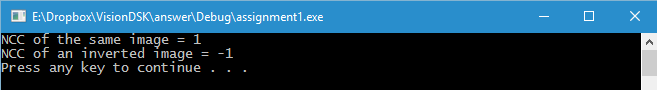
\includegraphics{Task1.png} 
\center
\caption {Output of the NCC for image(a) then image(b)}
\label{fig:copied_image}
\end{figure}

\section {Task 2: SAE}
I tested the SAE by first doing an SAE on the same image(a) and then doing an SAE on an inverse of the image(b). The expected output is 0 for image(a) since it is the same, and an extremely large number for image(b) as every element is the exact opposite of image(a). 

\subsection{Testing Code}
\begin{lstlisting}[language=C++]
Image task_2a = input_1;
std::cout << "SAE of the same image = " 
<< task_2a.getSAE(input_1) << std::endl;
// input parameters is the image to run
// the comparison against
Image task_2b = !input_1;
std::cout << "SAE of an inverted image= " 
<< task_2b.getSAE(input_1) << std::endl;
\end{lstlisting}

\subsection{Output}
\begin{figure}[h]
\center
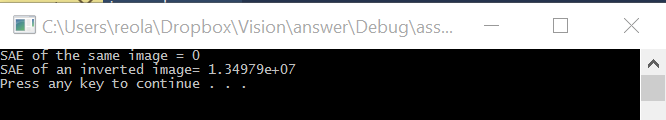
\includegraphics{Task2.PNG} 
\caption {Output of the NCC for image(a) then image(b)}
\label{fig:copied_image}
\end{figure}

\pagebreak

\section{Task 3: Intensity Histogram}
I computed three histogram images, image(a) has values between roughly 90 and 140 with 10 bins, image(b) has the same values with 5 bins, image(c) has values between roughly 190 and 240 with 10 bins.

\subsection{Testing Code}
\begin{lstlisting}[language=C++]
Image task_3a = input_1;
task_3a.getHistogram(10, "task3a.dat");
// input parameters are number of bins 
// and path of where to save the output file
std::cout << "Histogram 1 saved at \"/task3a.dat\"." << std::endl;

task_3a.getHistogram(5, "task3b.dat");
std::cout << "Histogram 2 saved at \"/task3b.dat\"." << std::endl;

Image task_3c = input_1 + 100;
task_3c.getHistogram(10, "task3c.dat");
std::cout << "Histogram 3 saved at \"/task3c.dat\"." << std::endl;
\end{lstlisting}

\subsection{Output}
\begin{figure}[h!]
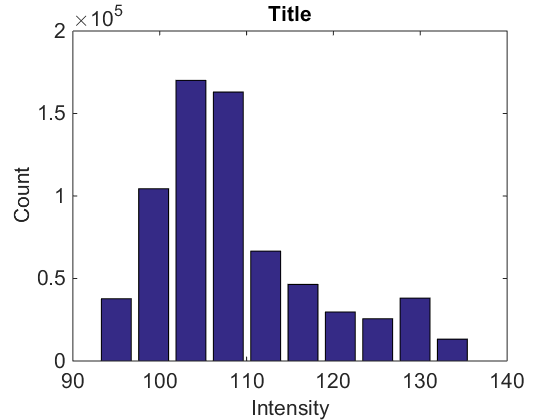
\includegraphics[scale=0.5]{task3a.png} 
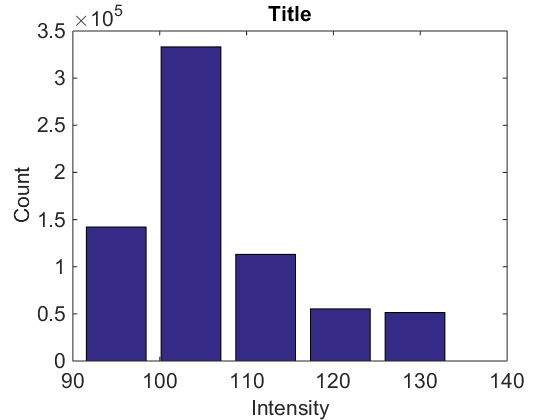
\includegraphics[scale=0.5]{task3b.png} 
\center
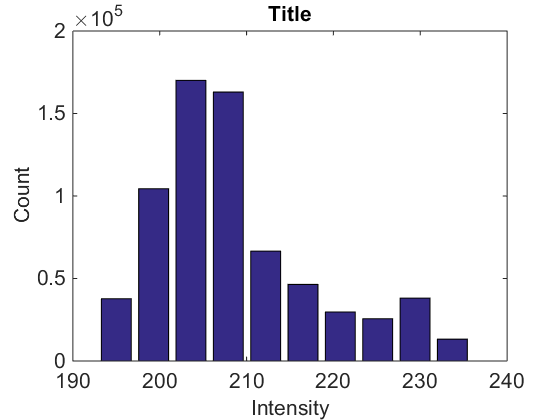
\includegraphics[scale=0.5]{task3c.png}
\caption {Left: image(a), Right: image(b), Bottom: image(c)}
\label{fig:copied_image}
\end{figure}


\pagebreak
\section{Task 4: Image Segmentation}
I used 120 for the threshold variable, that means that every variable at or above 120 should return 1 and anything below should return 0.
\subsection{Testing Code}
\begin{lstlisting}[language=C++]
Image task_4 = input_1 <= 120;
// paramter means any value less than 120
// will return 0 and anything at or above
// will return 1
task_4.savePGM("task4.pgm");
std::cout << "Threshold result saved at \"task4.pgm\"." << std::endl;
\end{lstlisting}
\subsection{Output}
\begin{figure}[h]
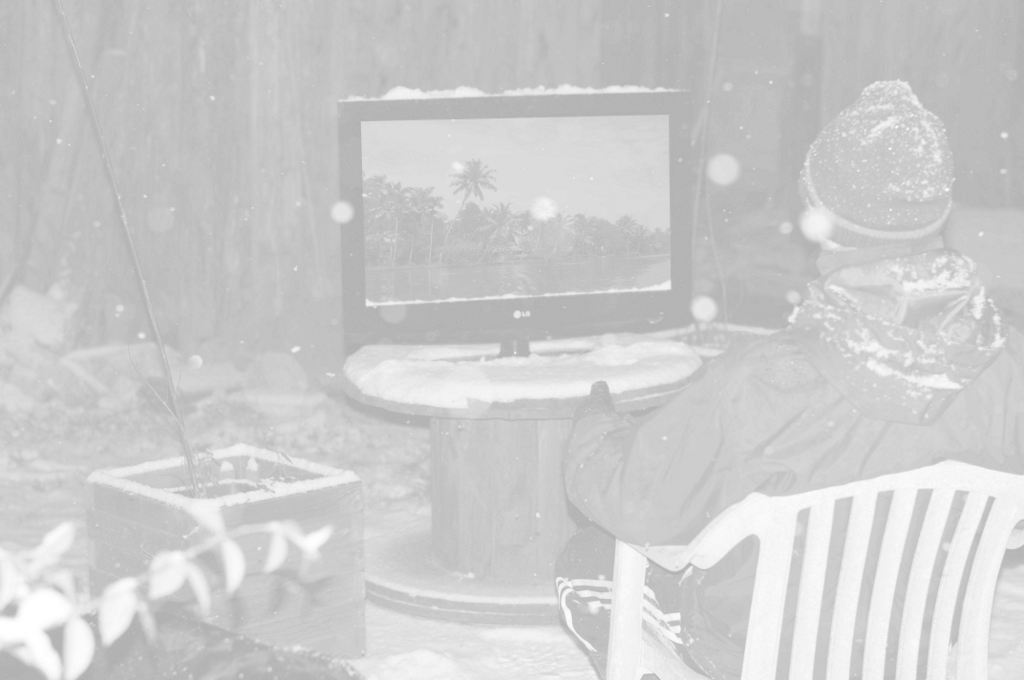
\includegraphics[scale=0.225]{snow.png}
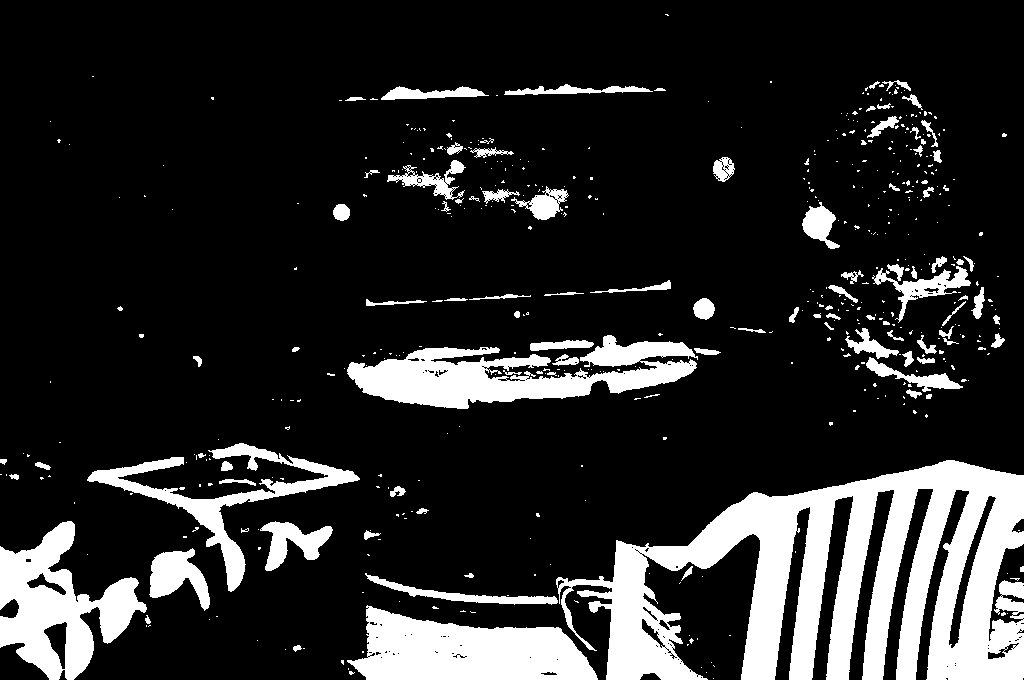
\includegraphics[scale=0.225]{task4.png} 
\caption {Image of threshold 120}
\label{fig:copied_image}
\end{figure}

\pagebreak

\section{Task 5: Image Blending}
I blended an Image by having 0.33 of the original image and 0.66 of double the original image.
\subsection{Testing Code}
\begin{lstlisting}[language=C++]
Image task_5 = input_1 * 2;
task_5 = task_5.blendImage(input_1, 0.33);
// parameters are an image to blend against
// and a parameter between 0 and 1
// which means the \% of each image to use
task_5.savePGM("task5.pgm");
std::cout << "Blending result saved at \"task5.pgm\"." << std::endl;
\end{lstlisting}

\subsection{Output}
\begin{figure}[h]
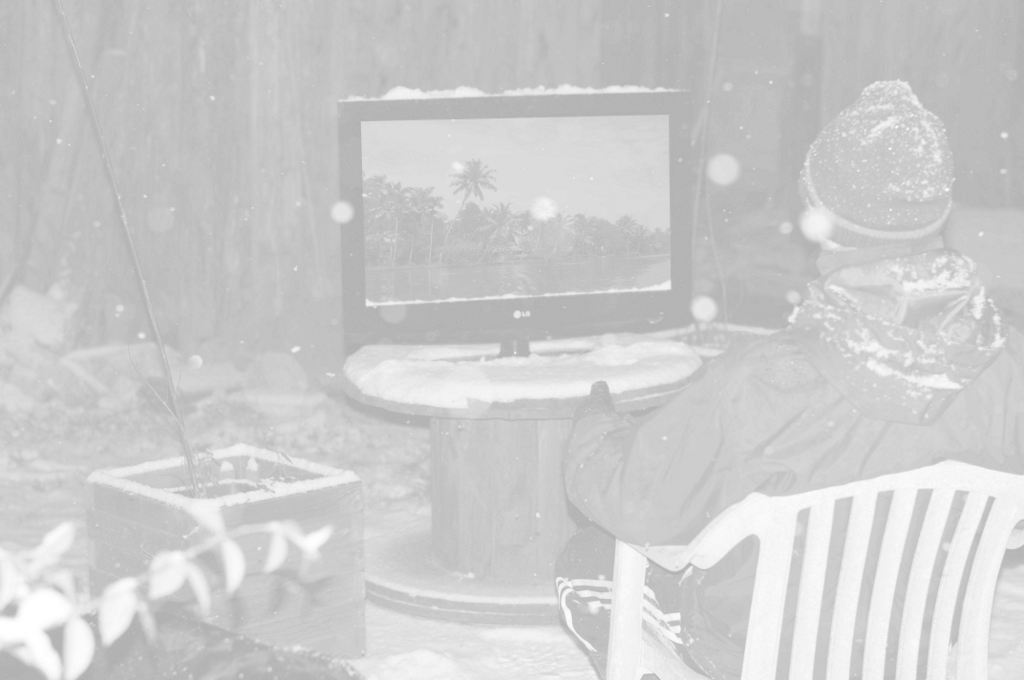
\includegraphics[scale=0.225]{snow.png}
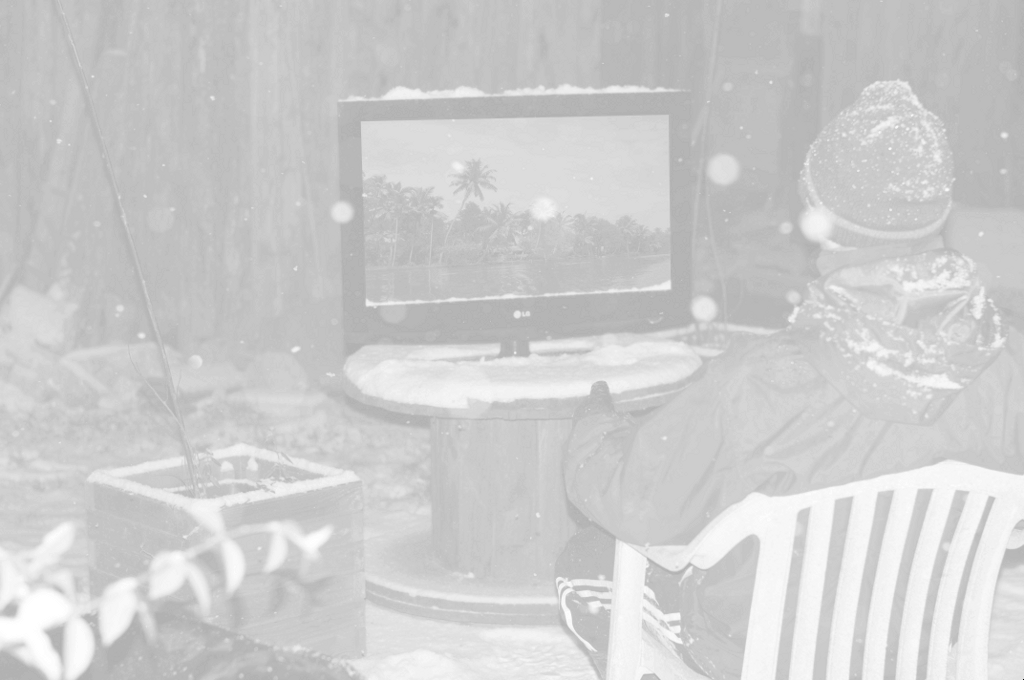
\includegraphics[scale=0.225]{task5.png} 
\caption {Left: original image, Right: blend of 0.66 of the original and 0.33 of double the original}
\label{fig:copied_image}
\end{figure}

\pagebreak

\section{Task 6: Resize Image}
I outputted three images: the original image, then the original image doubled, then the original image tripled.
\subsection{Testing Code}
\begin{lstlisting}[language=C++]
Image task_6a = input_1;
task_6a = task_6a.resizeImage(2);
// input parameter is the scale of the image, 
// input 2 = image * 2
task_6a.savePGM("task6a.pgm");

Image task_6b = input_1;
task_6b = task_6b.resizeImage(3);
task_6b.savePGM("task6b.pgm");
\end{lstlisting}

\subsection{Output}
\begin{figure}[h]
\center
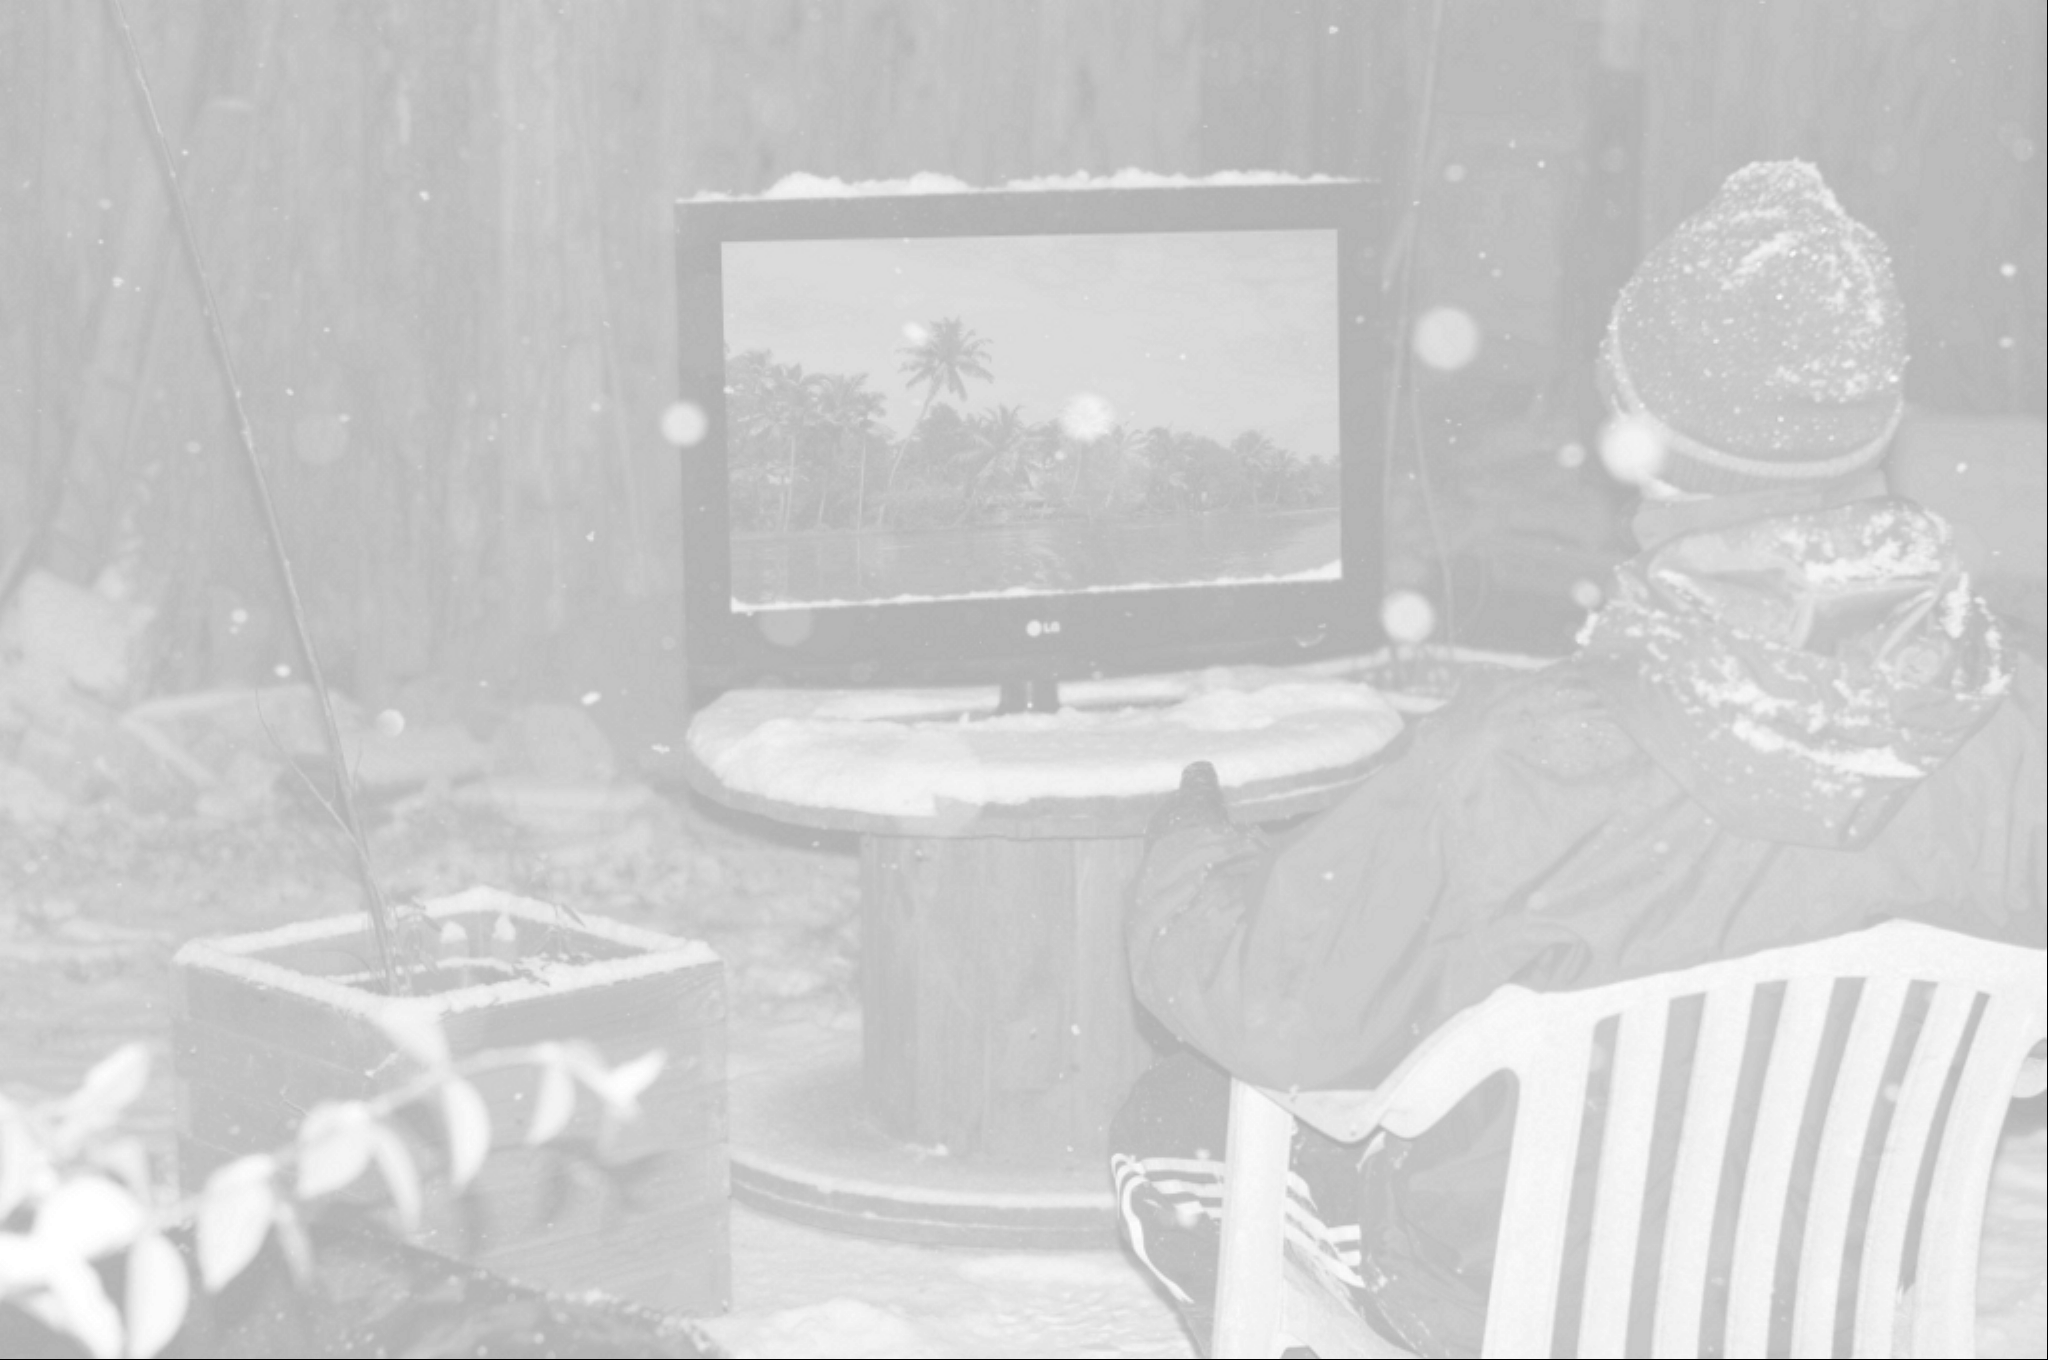
\includegraphics[scale=0.025]{task6a.png} 
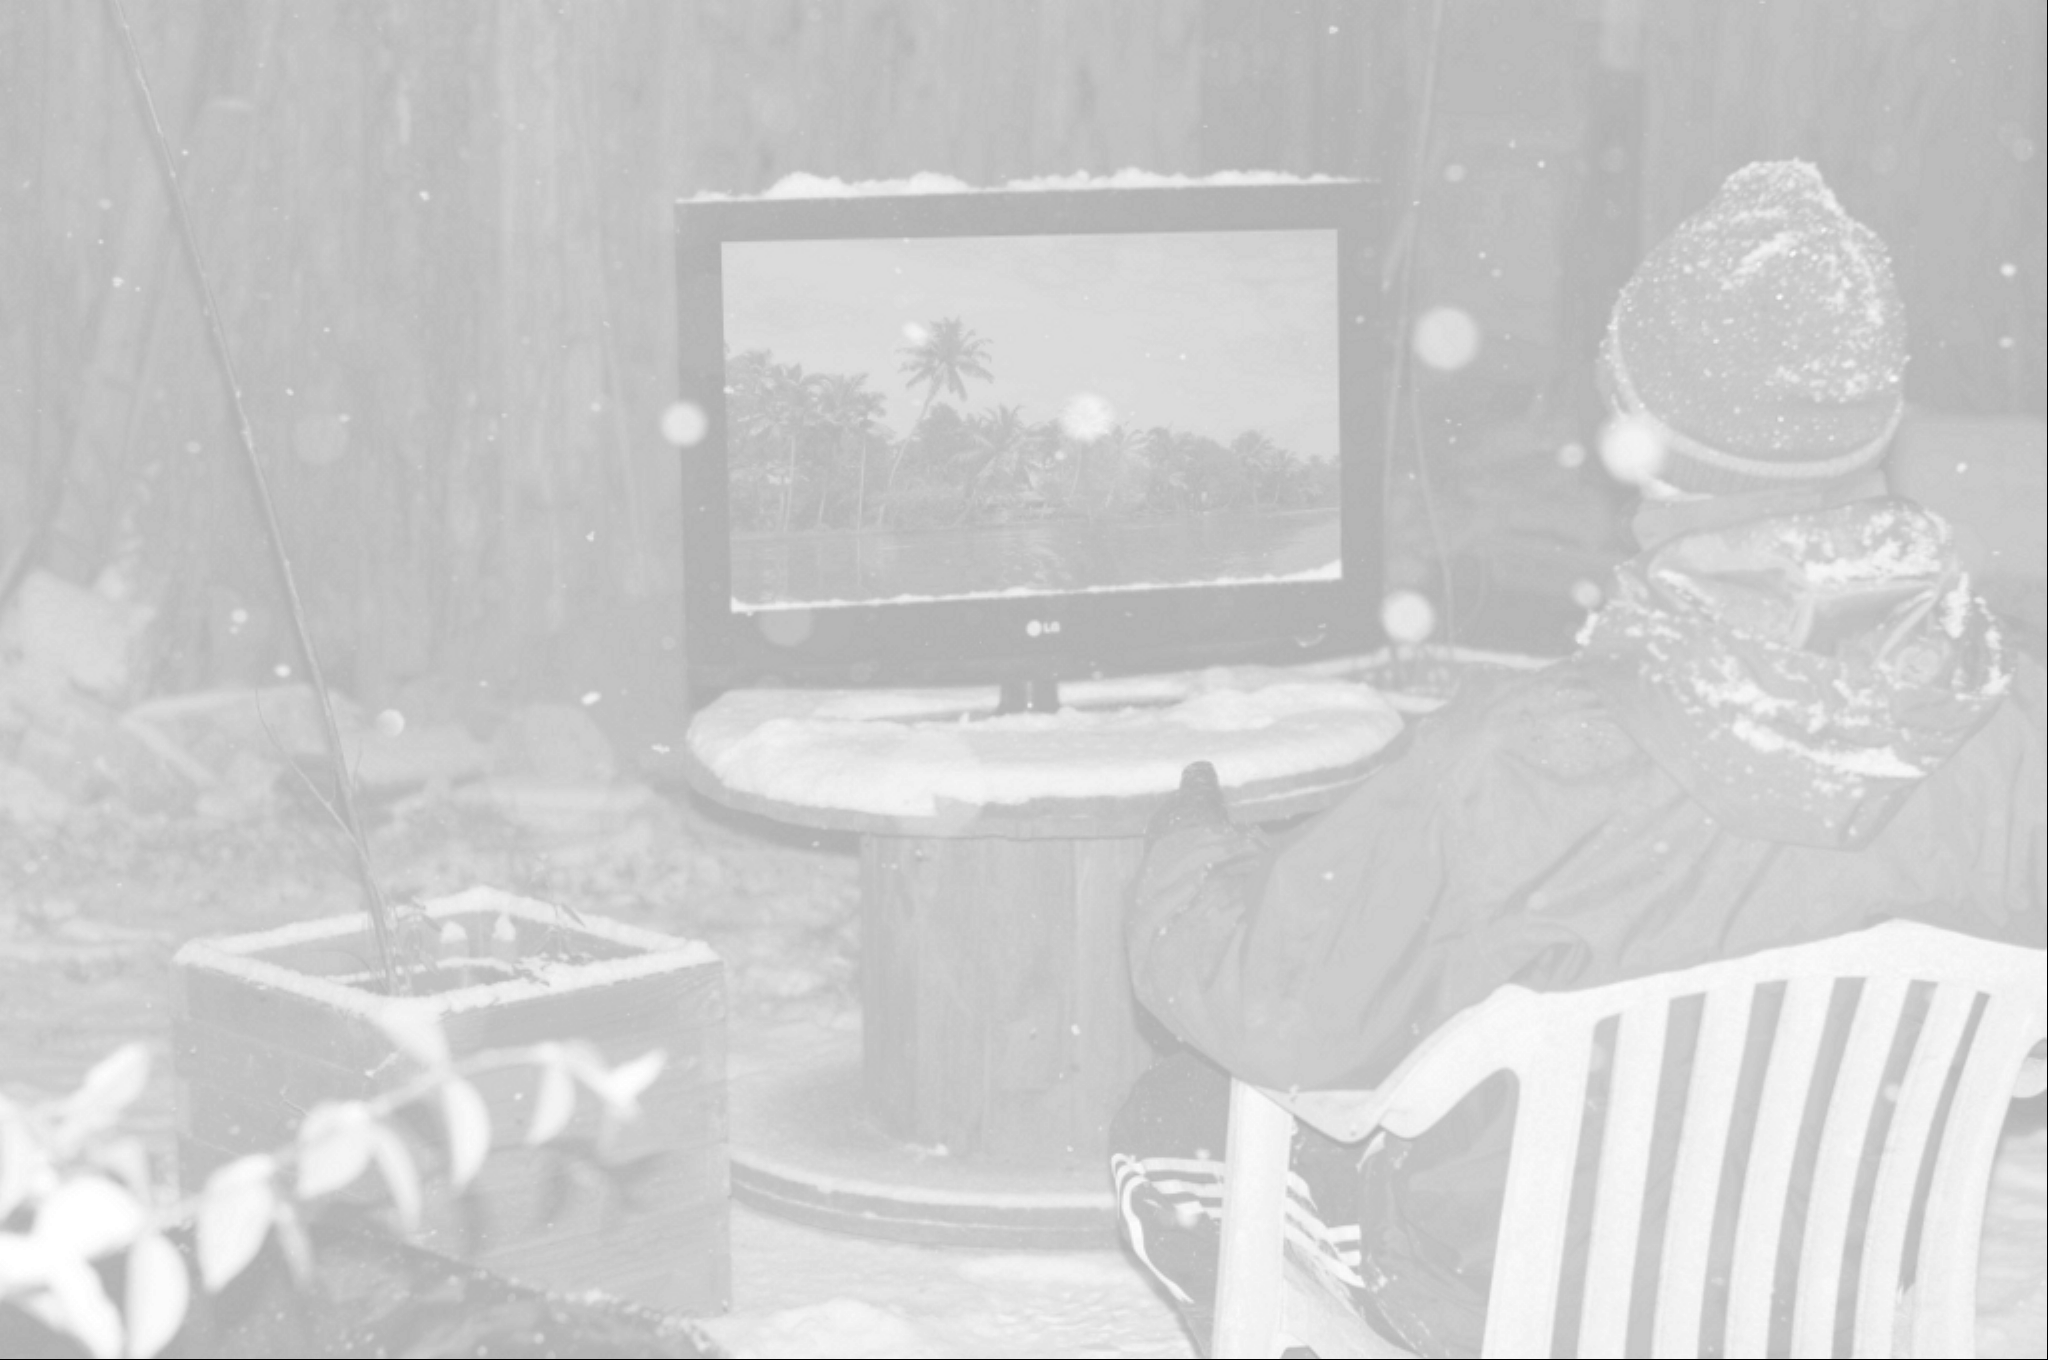
\includegraphics[scale=0.05]{task6a.png} 
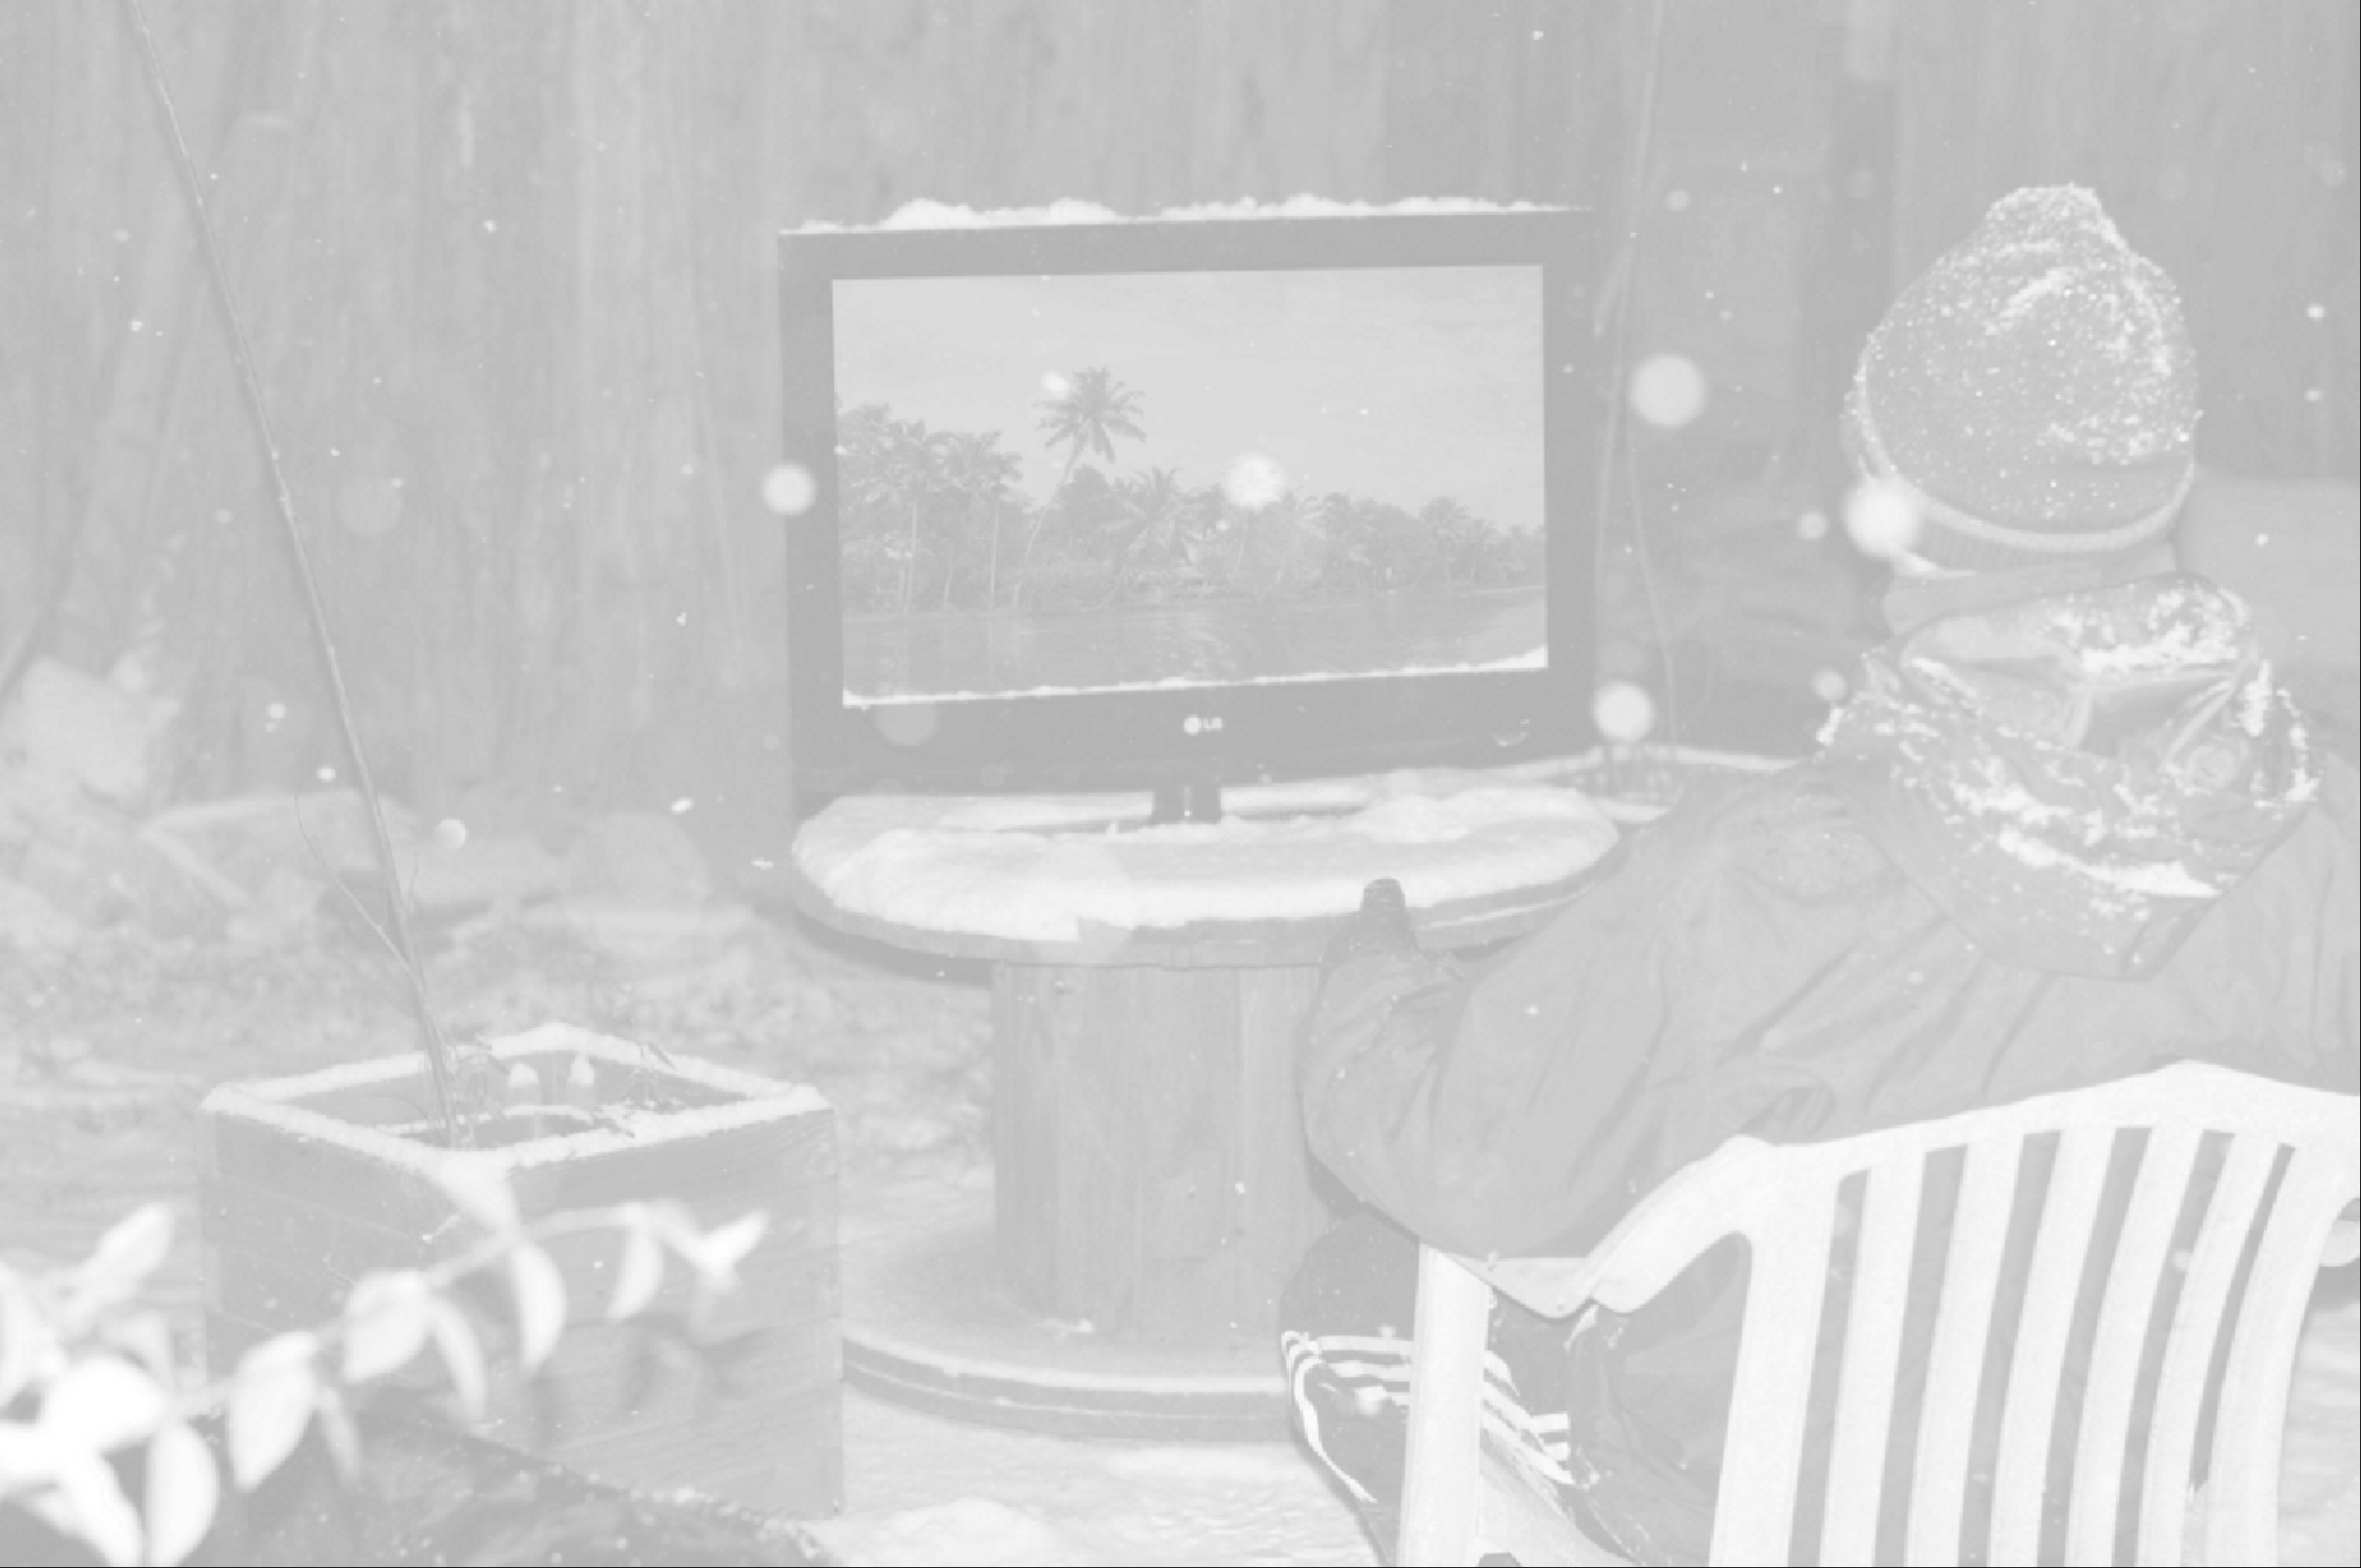
\includegraphics[scale=0.05]{task6b.png} 
\caption {Left: original, Center: original doubled, Right: original tripled}
\label{fig:copied_image}
\end{figure}

\pagebreak

\section{Task 7: Median Filter}
\subsection{Testing Code}
\begin{lstlisting}[language=C++]
Image task_7 = input_1;
task_7 = task_7.useMedianFilter();
task_7.savePGM("task7.pgm");
\end{lstlisting}

\subsection{Output}
\begin{figure}[h]
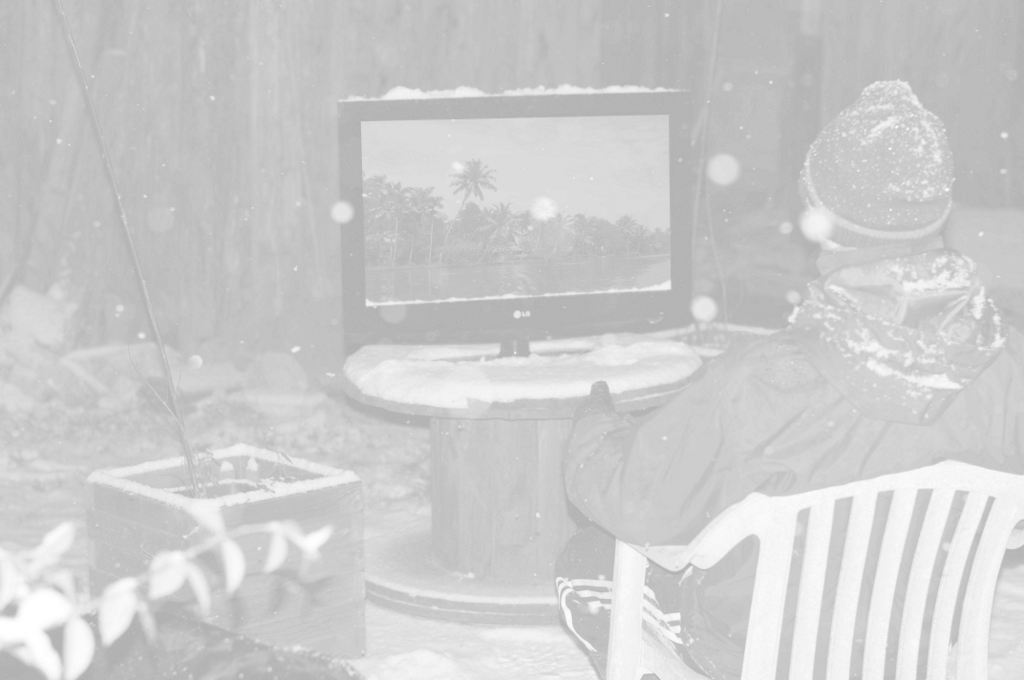
\includegraphics[scale=0.225]{snow.png}
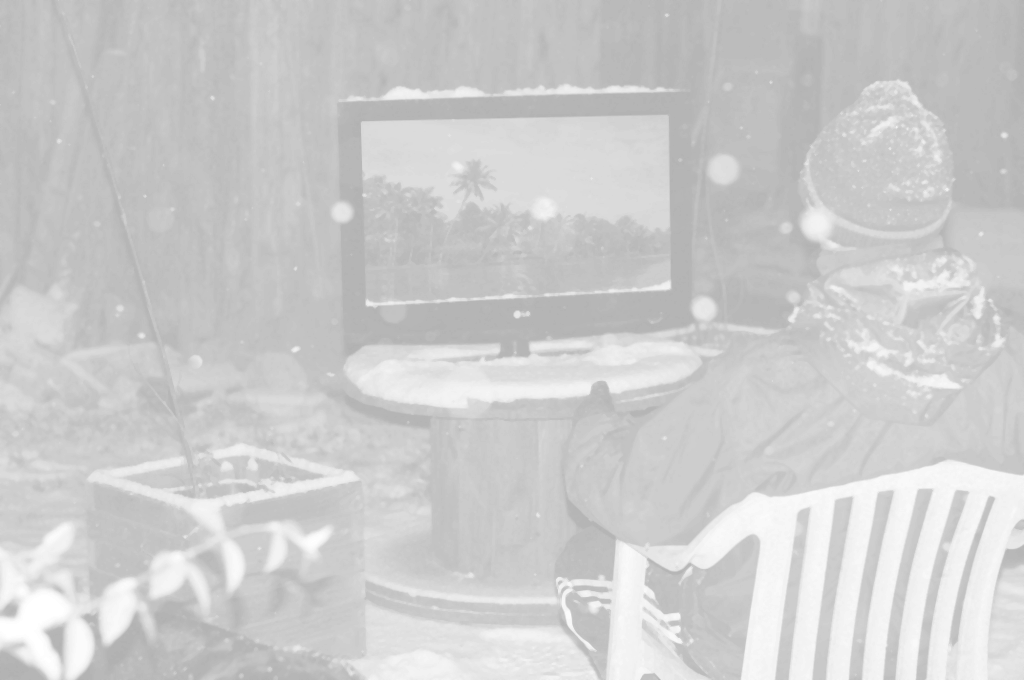
\includegraphics[scale=0.225]{task7.png} 
\caption {Left: original image, Right: original image after a median filter}
\label{fig:copied_image}
\end{figure}

\pagebreak

\section{Task 8: Spacial Convolution}
\subsection{Testing Code}
\begin{lstlisting}[language=C++]
Image task_8 = input_1;
std::vector<int> task_8_filter = { 1, 1, 1, 0, 0, 0, -1, -1, -1 };
// filter first element is 0,0, last element is 3,3
task_8 = task_8.useSpacialConvolution(task_8_filter);
// input the filter as a vector 
task_8.savePGM("task8.pgm");
\end{lstlisting}

\subsection{Output}
\begin{figure}[h]
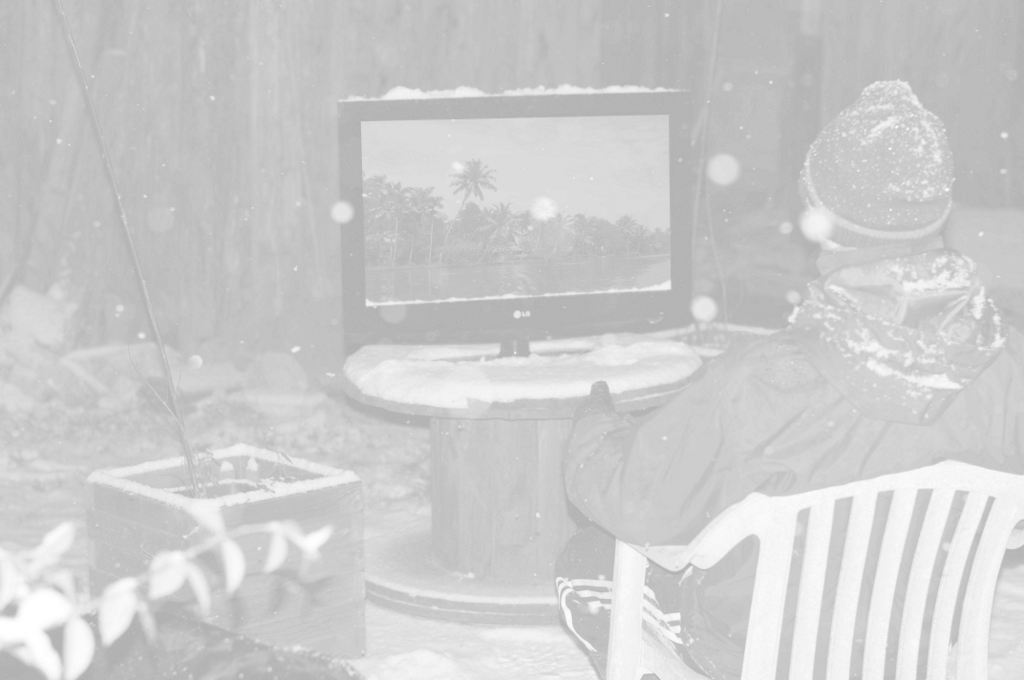
\includegraphics[scale=0.225]{snow.png}
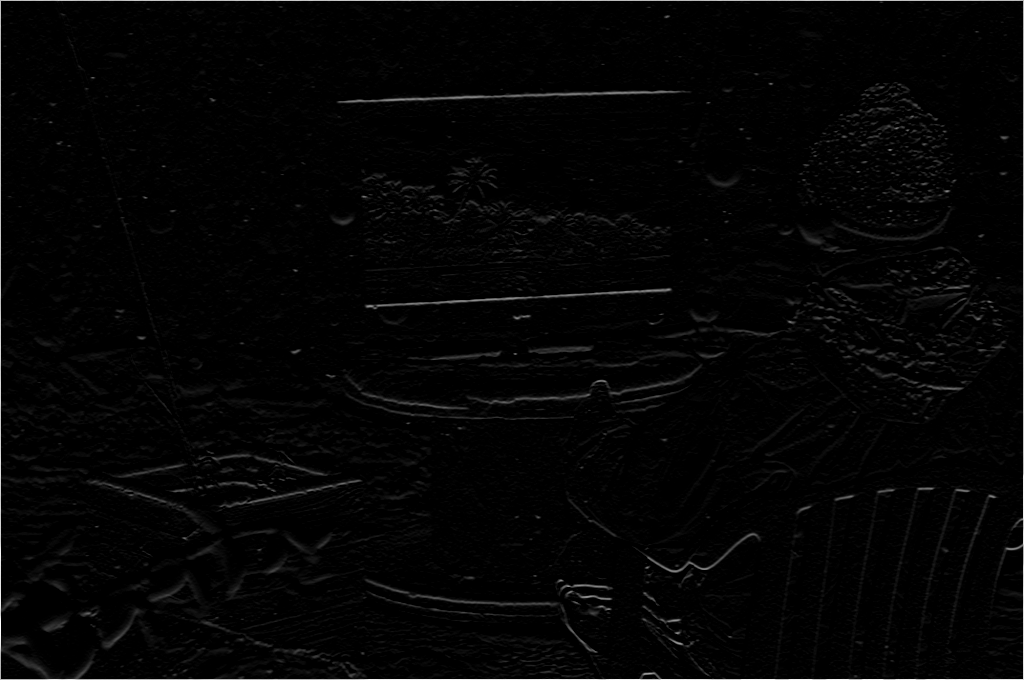
\includegraphics[scale=0.225]{task8.png} 
\caption {Left: original image, Right: original image after the inputted filter}
\label{fig:copied_image}
\end{figure}

\pagebreak

\section{Task 9: Preset Kernel}
\subsection{Testing Code}
\begin{lstlisting}[language=C++]
//Task 9a: Edge detection
Image task_9_a = input_1;
task_9_a = task_9_a.detectEdges();
task_9_a.savePGM("task9a.pgm");

//Task 9b: Sharpen
Image task_9_b = input_1;
task_9_b = task_9_b.sharpenImage();
task_9_b.savePGM("task9b.pgm");

//Task 9c: Box blur
Image task_9_c = input_1;
task_9_c = task_9_c.useBoxBlurFilter();
task_9_c.savePGM("task9c.pgm");

// Task 9d: Gaussian Blur
Image task_9_d = input_1;
task_9_d = task_9_d.useGaussianFilter();
task_9_d.savePGM("task9d.pgm");
\end{lstlisting}

\subsection{Output}
\begin{figure}[h]
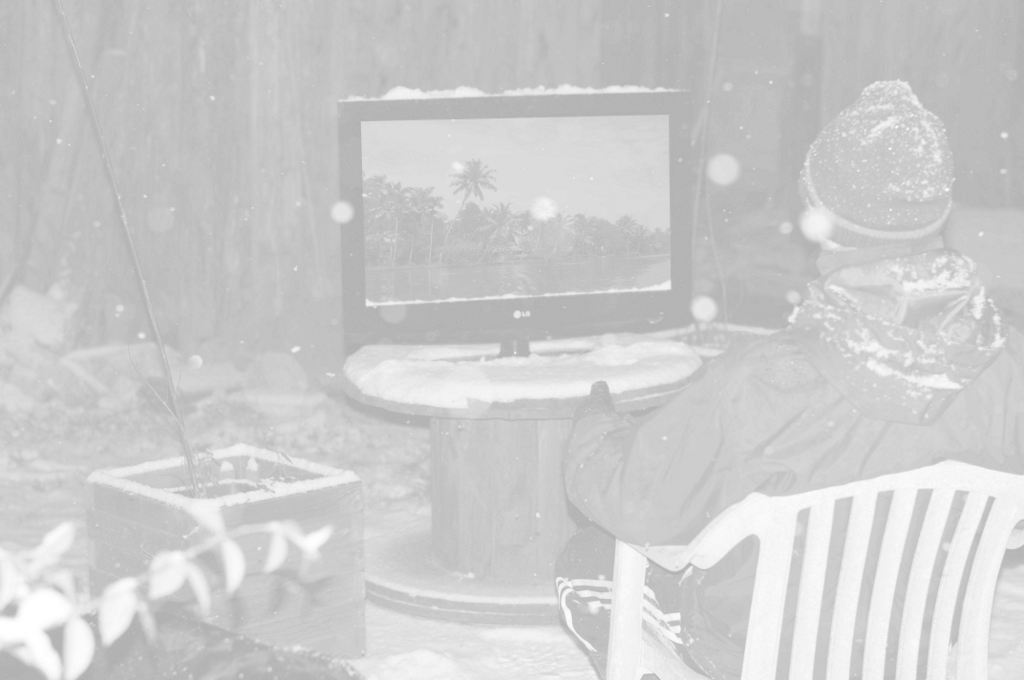
\includegraphics[scale=0.45]{snow.png}
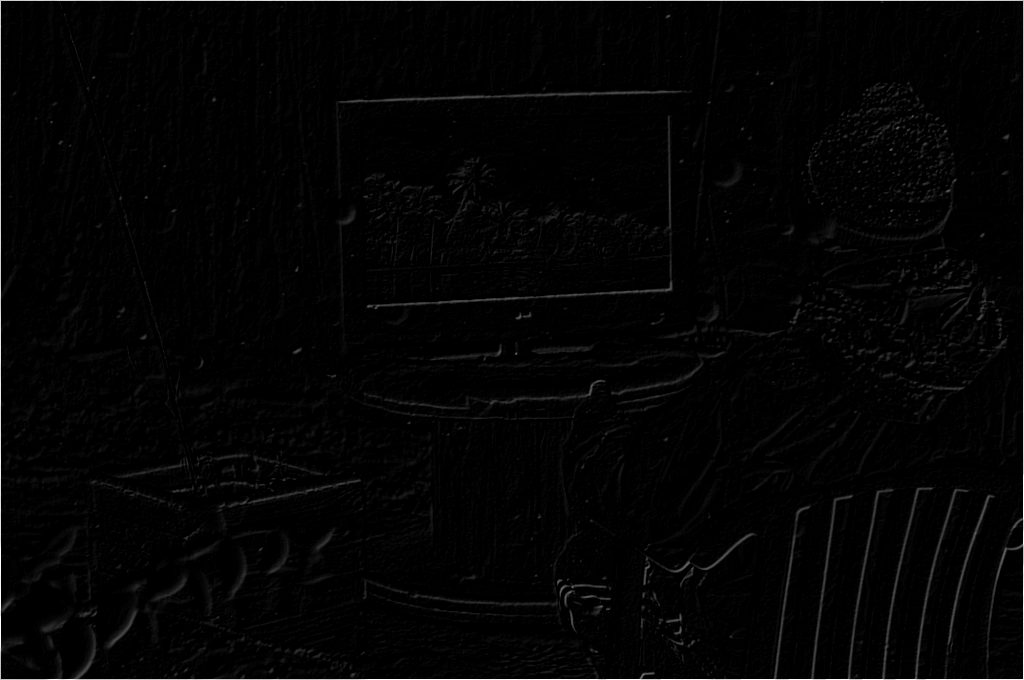
\includegraphics[scale=0.225]{task9a.png} 
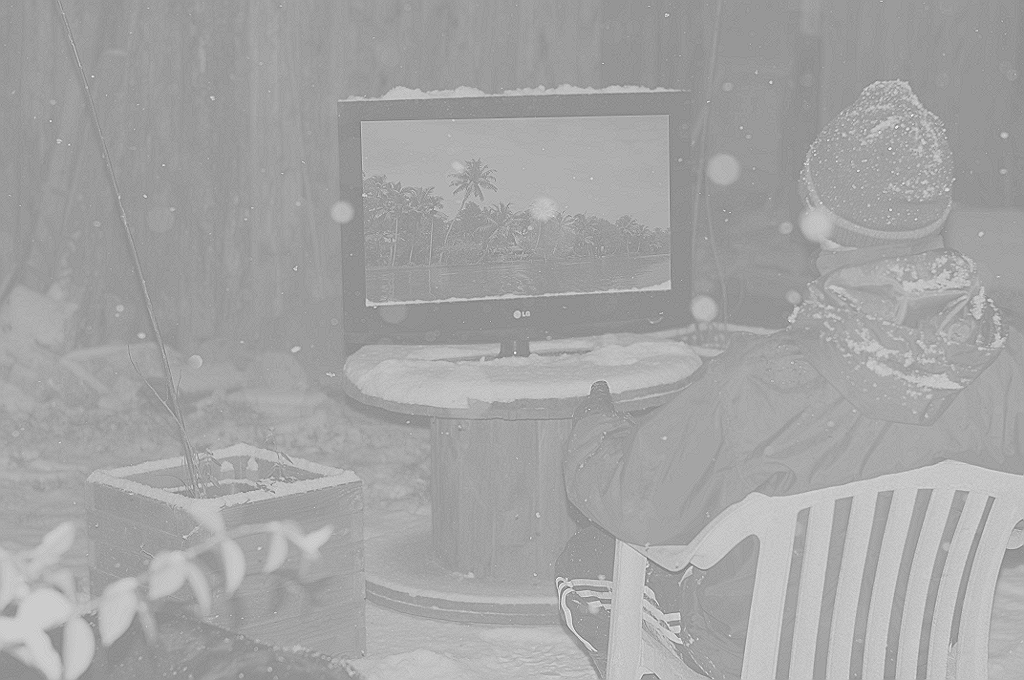
\includegraphics[scale=0.225]{task9b.png} 
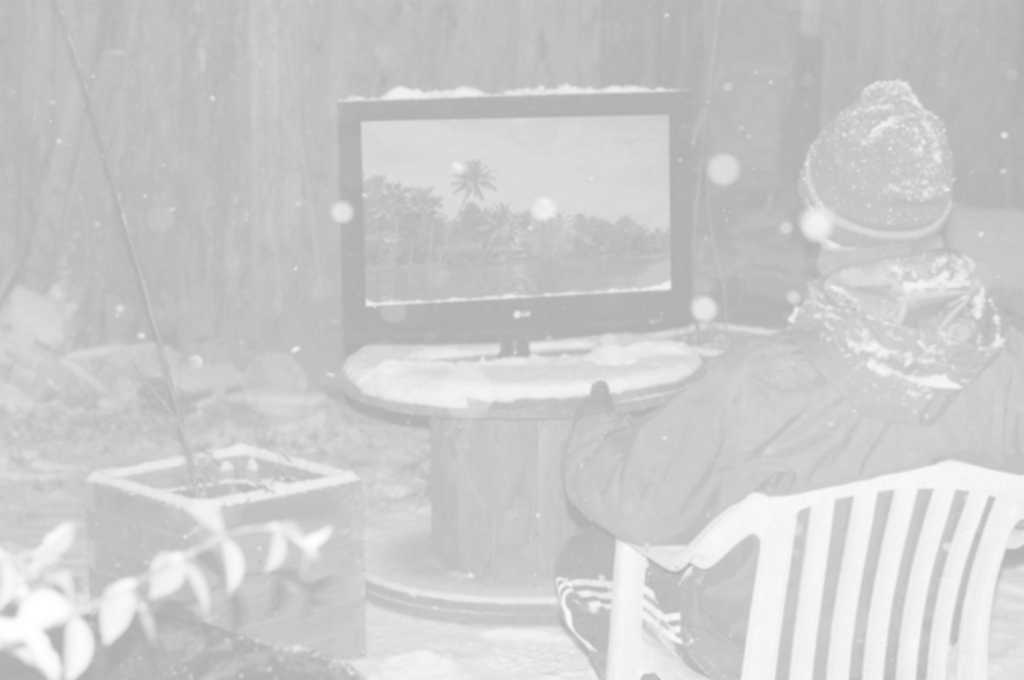
\includegraphics[scale=0.225]{task9c.png} 
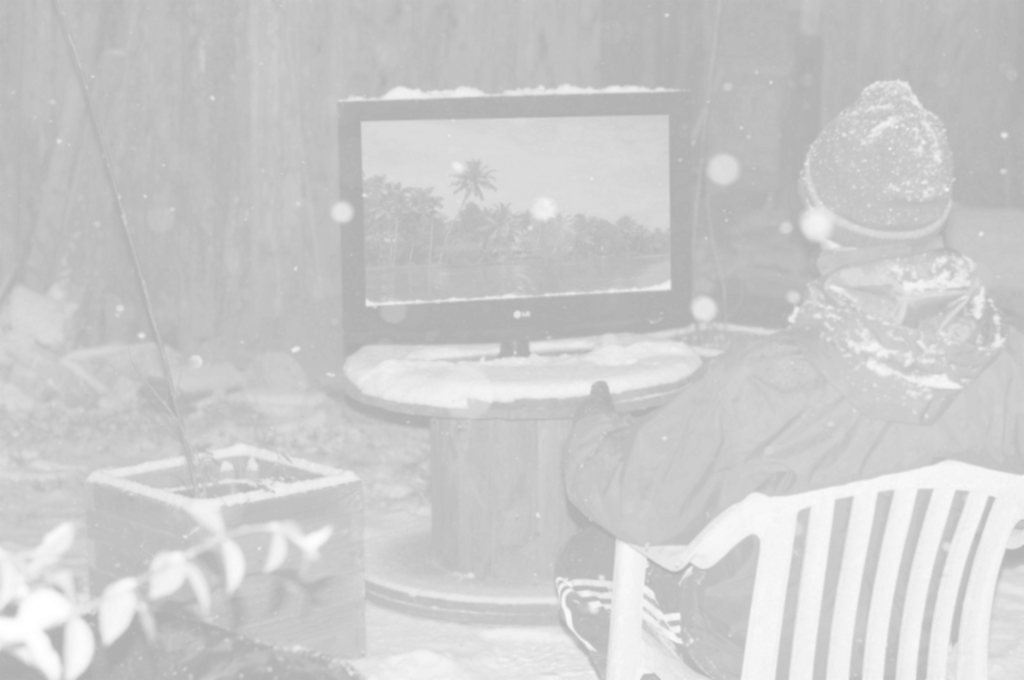
\includegraphics[scale=0.225]{task9d.png} 
\caption {Top Left to Bottom Right: original, edge detection, sharpen, box blur, gaussian blur}
\label{fig:copied_image}
\end{figure}

\pagebreak



% End the document
\end{document} 